\documentclass{standalone}
\usepackage{tikz}
\usetikzlibrary{automata,positioning,arrows,calc}
\tikzset{node distance=4cm,
	every state/.style={
		semithick,
		initial text={},
		%double distance=2pt,
		every edge/.style={
			draw,->,>=stealth',
			%auto,
			semithick
		}
	}
}

\begin{document}
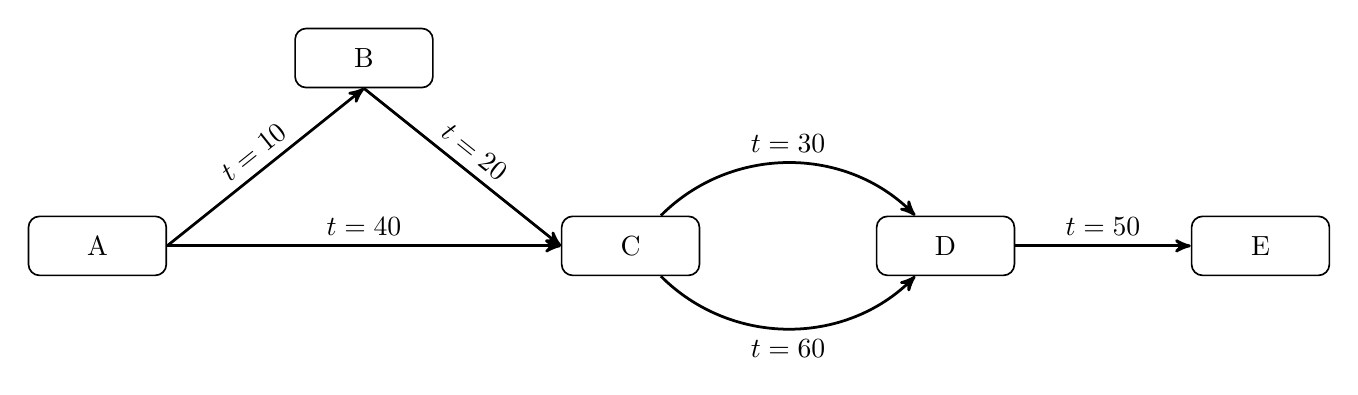
\begin{tikzpicture}[->,>=stealth',auto,semithick,line width=0.35mm]
		\tikzset{every state/.append style={rectangle,rounded corners,minimum height=0.75cm,minimum width=1.75cm}}
		\node[state] (1) {A};
		\node[state,right=1cm and 5cm of 1] (3) {C};
		\node[state,above=2cm] at ($(1)!0.5!(3)$) (2) {B};
		\node[state,right of=3] (4) {D};
		\node[state,right of=4] (5) {E};
		
		\path (1.east) edge node[above,sloped] {$t=10$ } (2.south)
		(1.east) edge node[above,sloped] {$t=40$} (3.west)
		(2.south) edge node[above,sloped] {$t=20$} (3.west)
		(3) edge[bend left=45] node[above,sloped] {$t=30$} (4)
		(3) edge[bend right=45] node[below,sloped] {$t=60$ } (4)
		(4) edge node[above,sloped] {$t=50$ } (5);
	\end{tikzpicture}
\end{document}
